\documentclass[tikz,border=10pt]{standalone}
\usepackage{amssymb} % for \subset
\usepackage{pgf,tikz,pgfplots,tkz-euclide}
\usepackage{tikz-3dplot}
\pgfplotsset{compat=1.15}
\usepackage{mathrsfs}
\usepackage{amsmath}
\allowdisplaybreaks[4]
\usetikzlibrary{arrows,arrows.meta,angles,quotes,automata,math}
\usetikzlibrary{calc,fadings,decorations.pathreplacing}
\usetikzlibrary{shadings,intersections}
\usetikzlibrary{3d}
\usetikzlibrary{hobby}
%\usepackage{amsthm}
\usepackage{wrapfig}
\usepackage{gensymb}
\usepackage{subfigure} 
\usepackage{physics}
\usepackage{diagbox}

\begin{document}

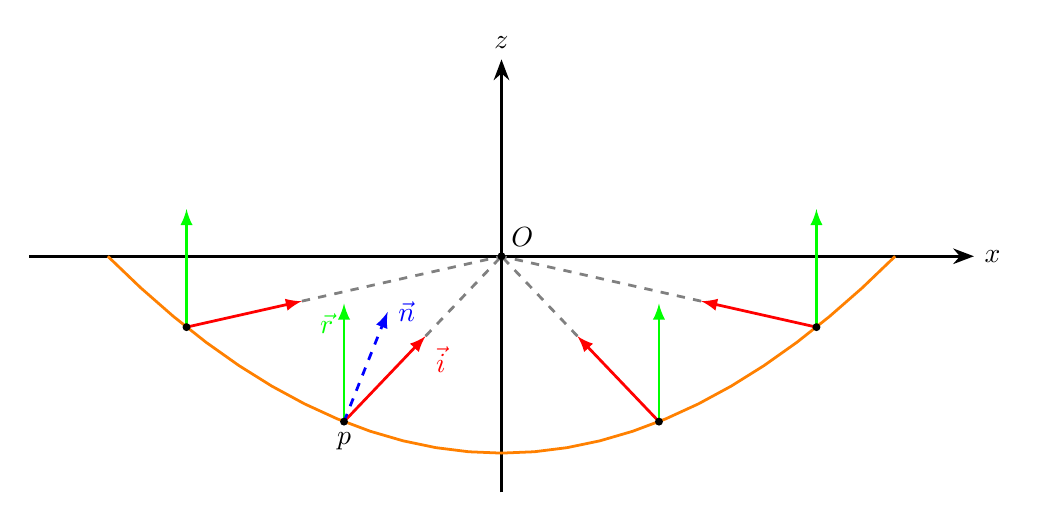
\begin{tikzpicture}[scale=5,domain=-1:1]
\coordinate [label=above right:$O$] (O) at (0,0);
\coordinate (P) at (-0.4,-0.42);
\coordinate (P1) at (-0.4,-0.12);
\coordinate (P2) at (-0.193, -0.203);
\coordinate (P3) at (-0.289, -0.141);
\coordinate (Q) at (-0.8,-0.18);
\coordinate (Q1) at (-0.8,0.12);
\coordinate (Q2) at (-0.507, -0.114);
\coordinate (R) at (0.8,-0.18);
\coordinate (R1) at (0.8,0.12);
\coordinate (R2) at (0.507, -0.114);
\coordinate (S) at (0.4,-0.42);
\coordinate (S1) at (0.4,-0.12);
\coordinate (S2) at (0.193, -0.203);
%\draw pic["$\theta$",draw,line width=1pt, angle eccentricity=1.5, angle radius=0.5cm] {angle=E--C--D};
\draw[-Stealth,line width=1pt] (-1.2,0) -- (1.2,0) node[right] {$x$};
\draw[-Stealth,line width=1pt] (0,-0.6) -- (0,0.5) node[above] {$z$};
\draw[color=orange,line width=1pt] plot (\x,{0.5*(\x)^2-0.5}) ;

\draw [line width=1pt,dash pattern=on 3pt off 3pt,gray] (P2) -- (O);
\draw [-latex,line width=1pt,red] (P) -- (P2) node[below right] {$\vec{i}$};
\draw [-latex,line width=1pt,green] (P) -- (P1) node[below left] {$\vec{r}$};
\draw [-latex,dash pattern=on 3pt off 3pt,line width=1pt,blue] (P) node[below,black] {$p$} -- (P3) node[right] {$\vec{n}$};
\draw [line width=1pt,dash pattern=on 3pt off 3pt,gray] (S2) -- (O);
\draw [-latex,line width=1pt,red] (S) -- (S2);
\draw [-latex,line width=1pt,green] (S) -- (S1);
\draw [line width=1pt,dash pattern=on 3pt off 3pt,gray] (Q2) -- (O);
\draw [-latex,line width=1pt,red] (Q) -- (Q2);
\draw [-latex,line width=1pt,green] (Q) -- (Q1);
\draw [line width=1pt,dash pattern=on 3pt off 3pt,gray] (R2) -- (O);
\draw [-latex,line width=1pt,red] (R) -- (R2);
\draw [-latex,line width=1pt,green] (R) -- (R1);

\foreach \p in {O,P,Q,R,S}
	\fill[fill=black,draw=black,thick] (\p) circle (0.2pt);
\end{tikzpicture}

\end{document}